\documentclass{article}
\usepackage[T1]{fontenc}
\usepackage{fancyhdr}
\usepackage{extramarks}
\usepackage{amsmath}
\usepackage{amsthm}
\usepackage{amsfonts}
\usepackage{dsfont}
\usepackage{tikz}
\usepackage[plain]{algorithm}
\usepackage{algpseudocode}
\usepackage{graphicx}
\usepackage{listings}

\graphicspath{ {./../img} }

\usetikzlibrary{automata,positioning}

%
% Basic Document Settings
%

\topmargin=-0.45in
\evensidemargin=0in
\oddsidemargin=0in
\textwidth=6.5in
\textheight=9.0in
\headsep=0.25in

\linespread{1.1}

\pagestyle{fancy}
\lhead{\hmwkAuthorName}
\chead{\hmwkTitle}
\rhead{\hmwkClass}
\lfoot{\lastxmark}
\cfoot{\thepage}

\renewcommand\headrulewidth{0.4pt}
\renewcommand\footrulewidth{0.4pt}

\setlength\parindent{0pt}
\setlength{\parskip}{5pt}

%
% Homework Details
%   - Title
%   - Due date
%   - Class
%   - Section/Time
%   - Instructor
%   - Author
%

\newcommand{\hmwkTitle}{Quiz\ \#1}
\newcommand{\hmwkDueDate}{October 16, 2023}
\newcommand{\hmwkClass}{ECE 271A}
\newcommand{\hmwkClassInstructor}{Professor Vasconcelos}
\newcommand{\hmwkAuthorName}{\textbf{Ray Tsai}}
\newcommand{\hmwkPID}{A16848188}

%
% Title Page
%

\title{
    \vspace{2in}
    \textmd{\textbf{\hmwkClass:\ \hmwkTitle}}\\
    \normalsize\vspace{0.1in}\small{Due\ on\ \hmwkDueDate\ at 11:59pm}\\
    \vspace{0.1in}\large{\textit{\hmwkClassInstructor}} \\
    \vspace{3in}
}

\author{
  \hmwkAuthorName \\
  \vspace{0.1in}\small\hmwkPID
}
\date{}

%
% Various Helper Commands
%

% Useful for algorithms
\newcommand{\alg}[1]{\textsc{\bfseries \footnotesize #1}}

% For derivatives
\newcommand{\deriv}[1]{\frac{\mathrm{d}}{\mathrm{d}x} (#1)}

% For partial derivatives
\newcommand{\pderiv}[2]{\frac{\partial}{\partial #1} (#2)}

% Integral dx
\newcommand{\dx}{\mathrm{d}x}

% Probability commands: Expectation, Variance, Covariance, Bias
\newcommand{\Var}{\mathrm{Var}}
\newcommand{\Cov}{\mathrm{Cov}}
\newcommand{\Bias}{\mathrm{Bias}}
\newcommand*{\Z}{\mathbb{Z}}
\newcommand*{\Q}{\mathbb{Q}}
\newcommand*{\R}{\mathbb{R}}
\newcommand*{\C}{\mathbb{C}}
\newcommand*{\N}{\mathbb{N}}
\newcommand*{\prob}{\mathds{P}}
\newcommand*{\E}{\mathds{E}}

\begin{document}

\maketitle

\pagebreak

\section*{Part A}
Using the training data in {\fontfamily{qcr}\selectfont TrainingSamplesDCT\textunderscore8.mat}, what are reasonable estimates for the prior probabilities? \\

\textbf{\large Solution}

We assume that {\fontfamily{qcr}\selectfont TrainingSampleDCT\textunderscore FG} and 
{\fontfamily{qcr}\selectfont TrainingSampleDCT\textunderscore BG} represents a set of complete images collectively.
Then, given that there are $250$ rows in {\fontfamily{qcr}\selectfont TrainingSampleDCT\textunderscore FG}
and $1053$ rows in {\fontfamily{qcr}\selectfont TrainingSampleDCT\textunderscore BG},
we use the ratio of the size of samples to give an estimate for the prior probabilities, namely 
\[
  \prob_Y(cheetah) = \frac{250}{1053 + 250} \approx 19\%,
\]
\[
  \prob_Y(grass) = \frac{1053}{1053 + 250} \approx 81\%.
\]

\section*{Part B}
Using the training data in {\fontfamily{qcr}\selectfont TrainingSamplesDCT\textunderscore8.mat}, compute and plot the index histograms
$P_{X|Y}(x|cheetah)$ and $P_{X|Y}(x|grass)$. \\

\textbf{\large Solution}

We collect feature $X$, the position of the coefficient of the second largest magnitude, from each row vector and normalize it to 
obtained the index histogram for $P_{X|Y}(x|cheetah)$ and $P_{X|Y}(x|grass)$:
\begin{center}
  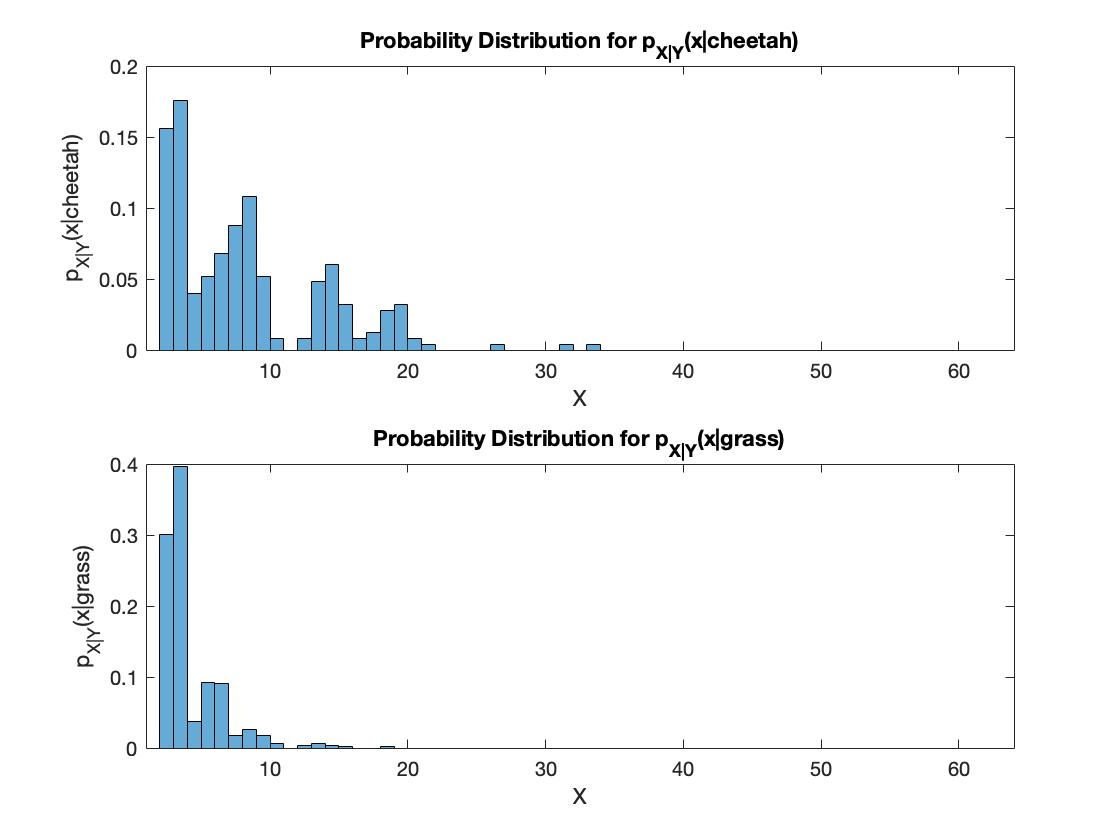
\includegraphics[scale=0.3]{probability_histogram}
\end{center}

\pagebreak

\section*{Part C}

For each block in the image {\fontfamily{qcr}\selectfont cheetah.bmp}, compute the feature $X$ (index of the DCT coefficient with
2nd greatest energy). Compute the state variable $Y$ using the minimum probability of error rule based
on the probabilities obtained in part a and b. Store the state in an array $A$. Using the commands {\fontfamily{qcr}\selectfont imagesc} 
and {\fontfamily{qcr}\selectfont colormap(gray(255))}, create a picture of that array. \\

\textbf{\large Solution}

Let $g(x)$ be our decision function. Assume our loss function 
$L[g(x), y] = \begin{cases}
  1, &g(x) \neq y \\
  0, &g(x) = y
\end{cases}$. 
By the minimum probability of error rule, the optimal decision function is
\begin{align*}
  g^*(x) 
  &= {\arg \max}_{i} \prob_{Y|X}(i | x) \\
  &= {\arg \max}_{i} \prob_{X|Y}(x | i)\prob_Y(i) \\
  &= \begin{cases}
    cheetah, &\frac{\prob_{X|Y}(grass | x)}{\prob_{X|Y}(cheetah | x)} < \frac{\prob_Y(cheetah)}{\prob_Y(grass)} \\
    grass, &\text{otherwise}
  \end{cases} \\
  &= \begin{cases}
    cheetah, &\frac{\prob_{X|Y}(grass | x)}{\prob_{X|Y}(cheetah | x)} < 0.24 \\
    grass, &\text{otherwise},
  \end{cases}
\end{align*}
for the 0-1 loss function. We then use function $g^*(x)$ to assign a state to each pixel and obtian 
our pridiction mask array $A$. Resulting picture of array $A$ is shown at the bottom of the page.

\section*{Part D}

The array $A$ contains a mask that indicates which blocks contain grass and which contain the
cheetah. Compare it with the ground truth provided in image {\fontfamily{qcr}\selectfont cheetah\textunderscore mask.bmp} and compute the probability of error of your algorithm. \\

\textbf{\large Solution}
By comparing our prediction with the truth, we calculate the error rate with the following formula
\[
  \text{Error rate} = \frac{\text{number of pixels of different values}}{\text{number of pixels}}.
\]
Results shown in the following figure.
\begin{center}
  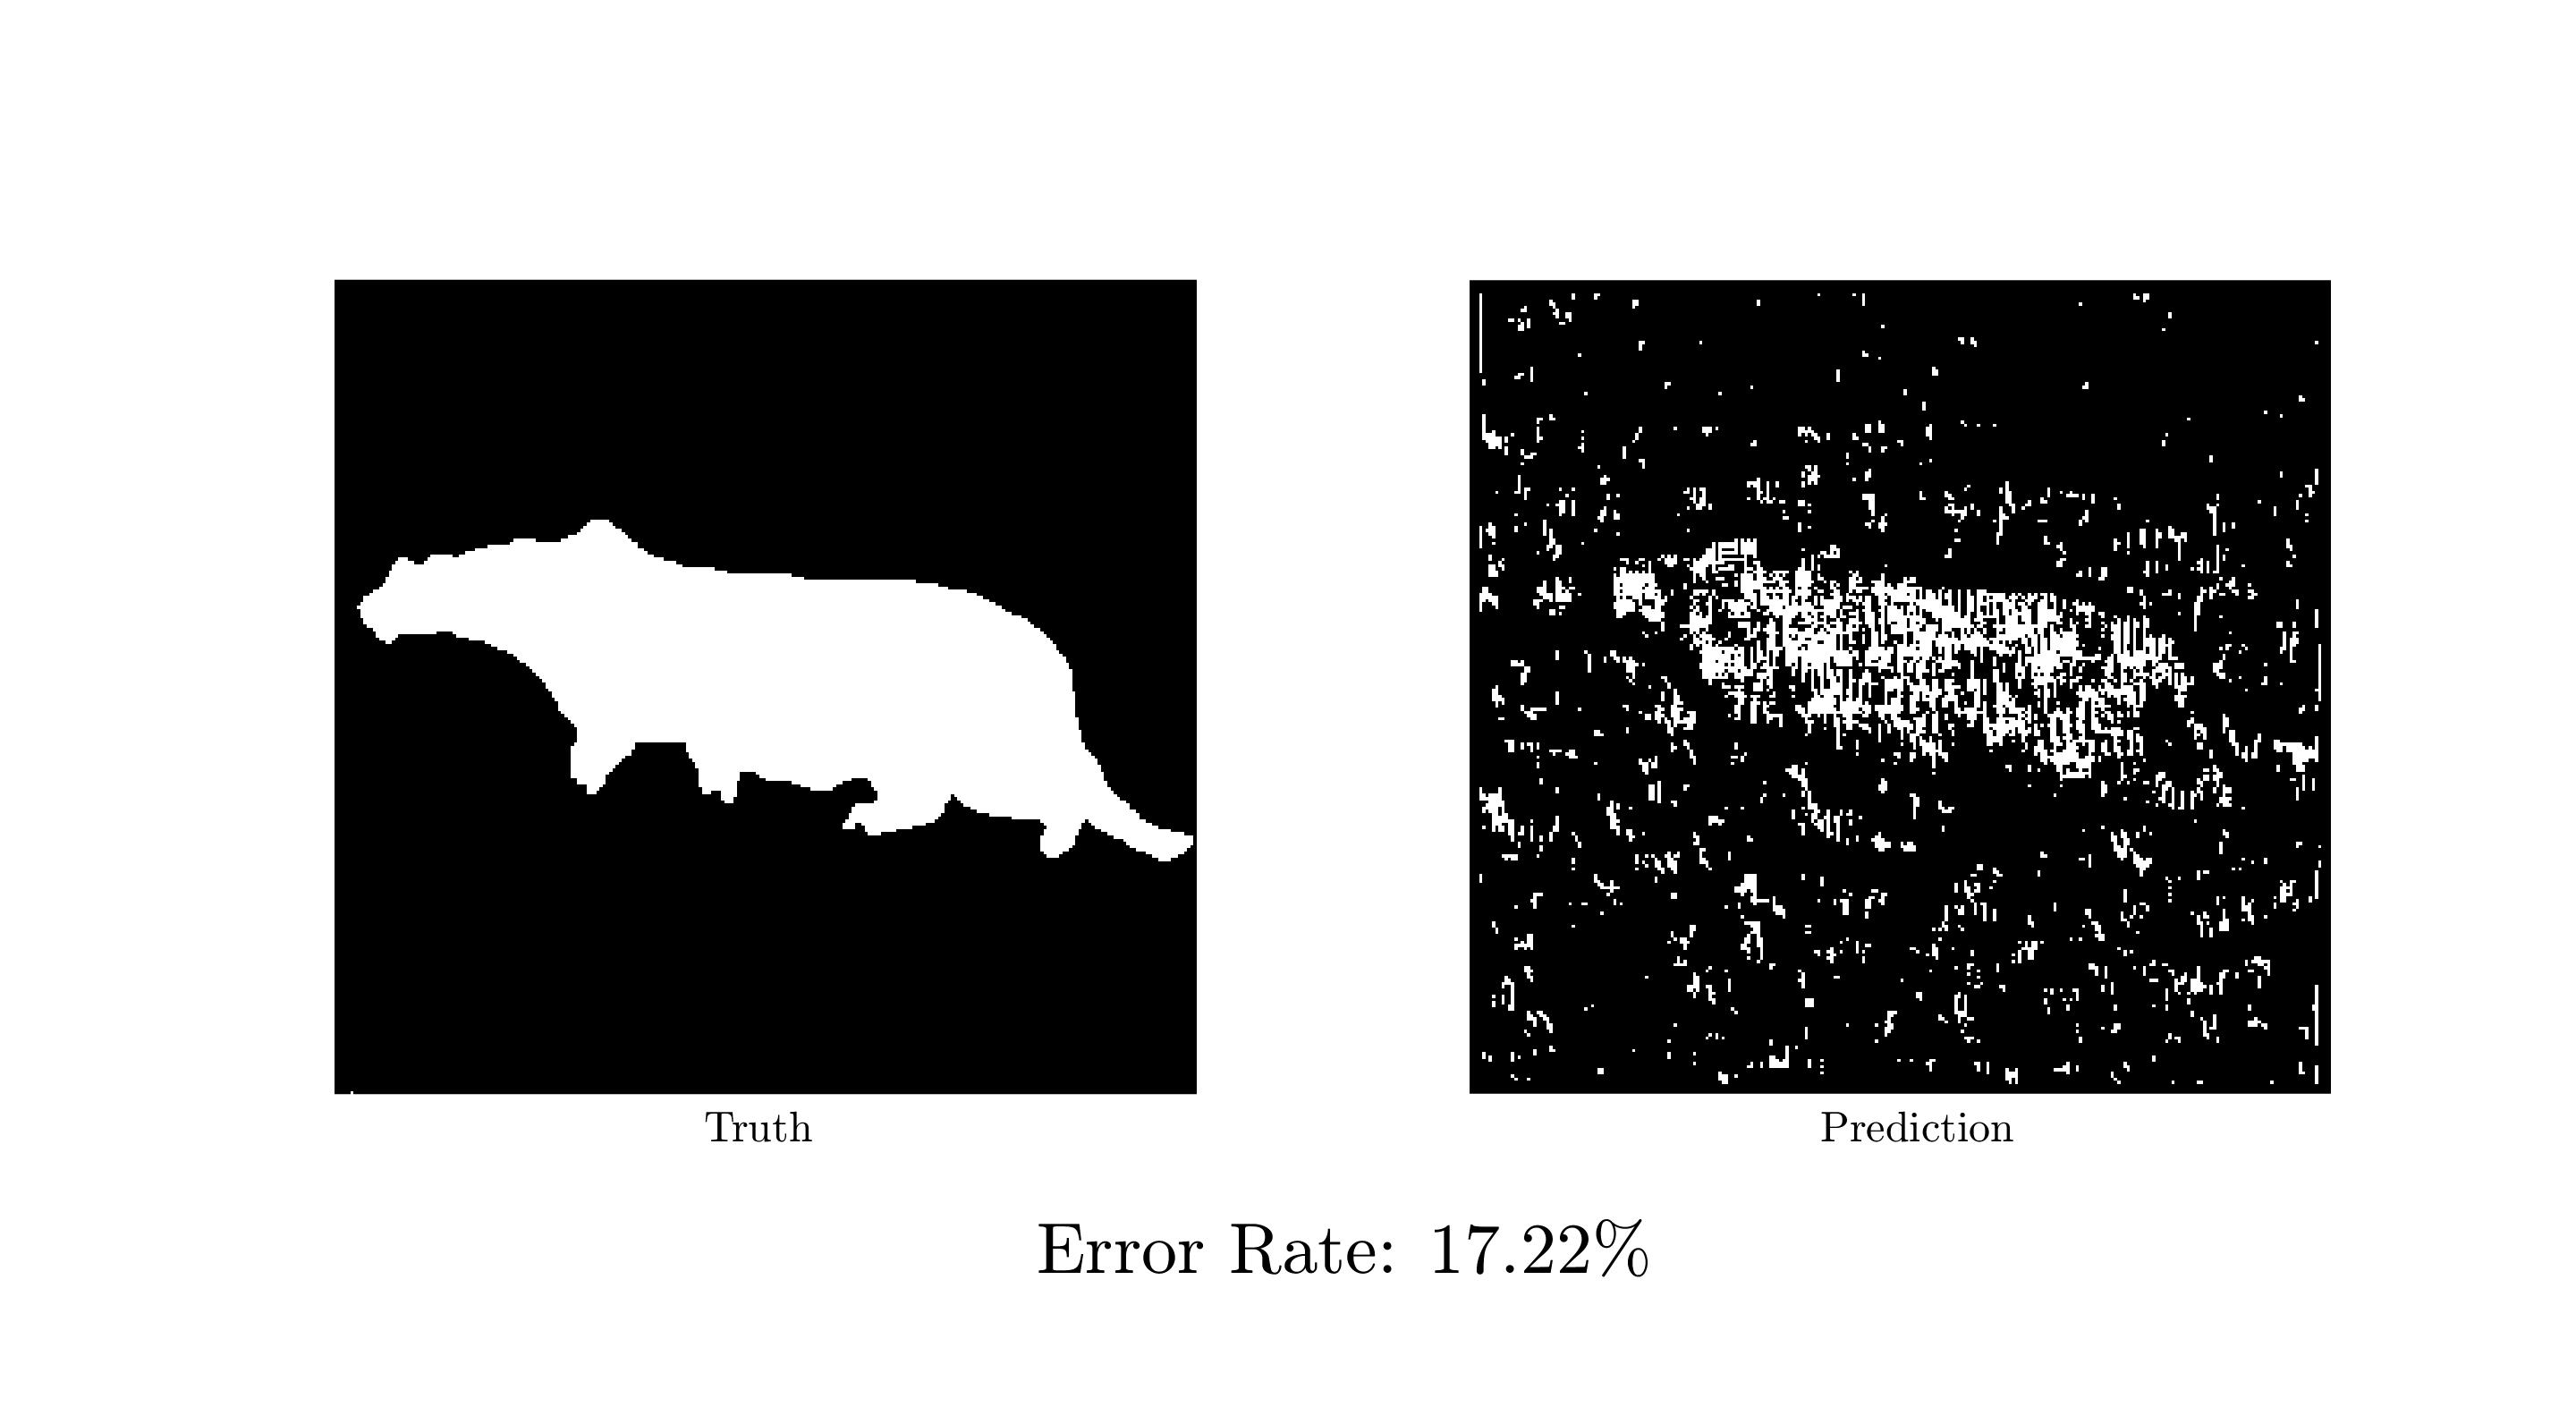
\includegraphics[scale=0.1]{comparison}
\end{center}

\section*{MATLAB Code}

\begin{lstlisting}[language=Matlab]
  load('../dataset/TrainingSamplesDCT_8.mat');
  zigzag = load('../dataset/Zig-Zag Pattern.txt');
  cheetah = imread('../dataset/cheetah.bmp');
  cheetah_mask = imread('../dataset/cheetah_mask.bmp');
  target = im2double(cheetah);
  mask = im2double(cheetah_mask);

  training_BG = TrainsampleDCT_BG;
  training_FG = TrainsampleDCT_FG;
  zigzag = zigzag + 1;

  [row_BG, col_BG] = size(training_BG);
  [row_FG, col_FG] = size(training_FG);
  [row_TG, col_TG] = size(target);

  padded_target = zeros(row_TG + 7, col_TG + 7);
  padded_target(5:4 + row_TG, 5:4 + col_TG) = target;

  % pick cheetah if (p(x | grass) / p(x | cheetah)) < threshold
  prior_BG = row_BG / (row_BG + row_FG);
  prior_FG = row_FG / (row_BG + row_FG);
  threshold = prior_FG / prior_BG;

  feature_BG = zeros(64, 1);
  feature_FG = zeros(64, 1);

  for r = 1:1:row_BG
      maxVal = max(training_BG(r));
      secVal = 0;
      secPos = 0;
      for c = 1:1:col_BG
          if (training_BG(r, c) < maxVal && training_BG(r, c) > secVal)
              secVal = training_BG(r, c);
              secPos = c;
          end
      end
      feature_BG(secPos) = feature_BG(secPos) + 1;
  end

  for r = 1:1:row_FG
      maxVal = max(training_FG(r));
      secVal = 0;
      secPos = 0;
      for c = 1:1:col_FG
          if (training_FG(r, c) < maxVal && training_FG(r, c) > secVal)
              secVal = training_FG(r, c);
              secPos = c;
          end
      end
      feature_FG(secPos) = feature_FG(secPos) + 1;
  end

  cprob_BG = feature_BG / sum(feature_BG);
  cprob_FG = feature_FG / sum(feature_FG);
  A = zeros(row_TG, col_TG);

  for r = 1:row_TG
      for c = 1:col_TG
          block = padded_target(r:r + 7, c:c + 7);
          dctBlock = abs(dct2(block));
          maxVal = max(max(dctBlock));
          secVal = 0;
          x = 0;
          for i = 1:8
              for j = 1:8
                  if dctBlock(i, j) < maxVal && dctBlock(i, j) > secVal
                      secVal = dctBlock(i, j);
                      x = zigzag(i, j);
                  end
              end
          end
          A(r, c) = int8(cprob_BG(x)/cprob_FG(x) <= threshold);
      end
  end

  subplot(1, 2, 1);
  imagesc(mask);
  axis off
  colormap(gray(255));
  axis equal tight;

  subplot(1, 2, 2);
  imagesc(A);
  axis off
  colormap(gray(255));
  axis equal tight;

  error = 0;
  for r = 1:row_TG
      for c = 1:col_TG
          if (A(r, c) ~= mask(r, c))
              error = error + 1;
          end
      end
  end
  error_rate = error / (row_TG * col_TG);
\end{lstlisting}

\end{document}